
The Write Back Stage is the last stage in the DLX pipeline and it is used to write the results, that can come from the memory (due to a load) or the computation of the ALU, into the File Register.
Since this DXL is a pipelined processor, the destination register is available when the instruction is decoded and must be propagated until the write back register is needed. For this purpose, inside the entire Datapath, there is a skewing network that is used to have the register index exactly when necessary. \newline\newline
We need to extract from the instruction itself, depending on its type, the destination address. The position on a 32 bit instruction of the destination address is the following (refer to \ref{section:inst_set}):
\begin{itemize}
    \itemsep0sp
    \item R-Type: [25...21]
    \item I-Type: [20...16]
\end{itemize}
\begin{figure}[H]   
    \centering
    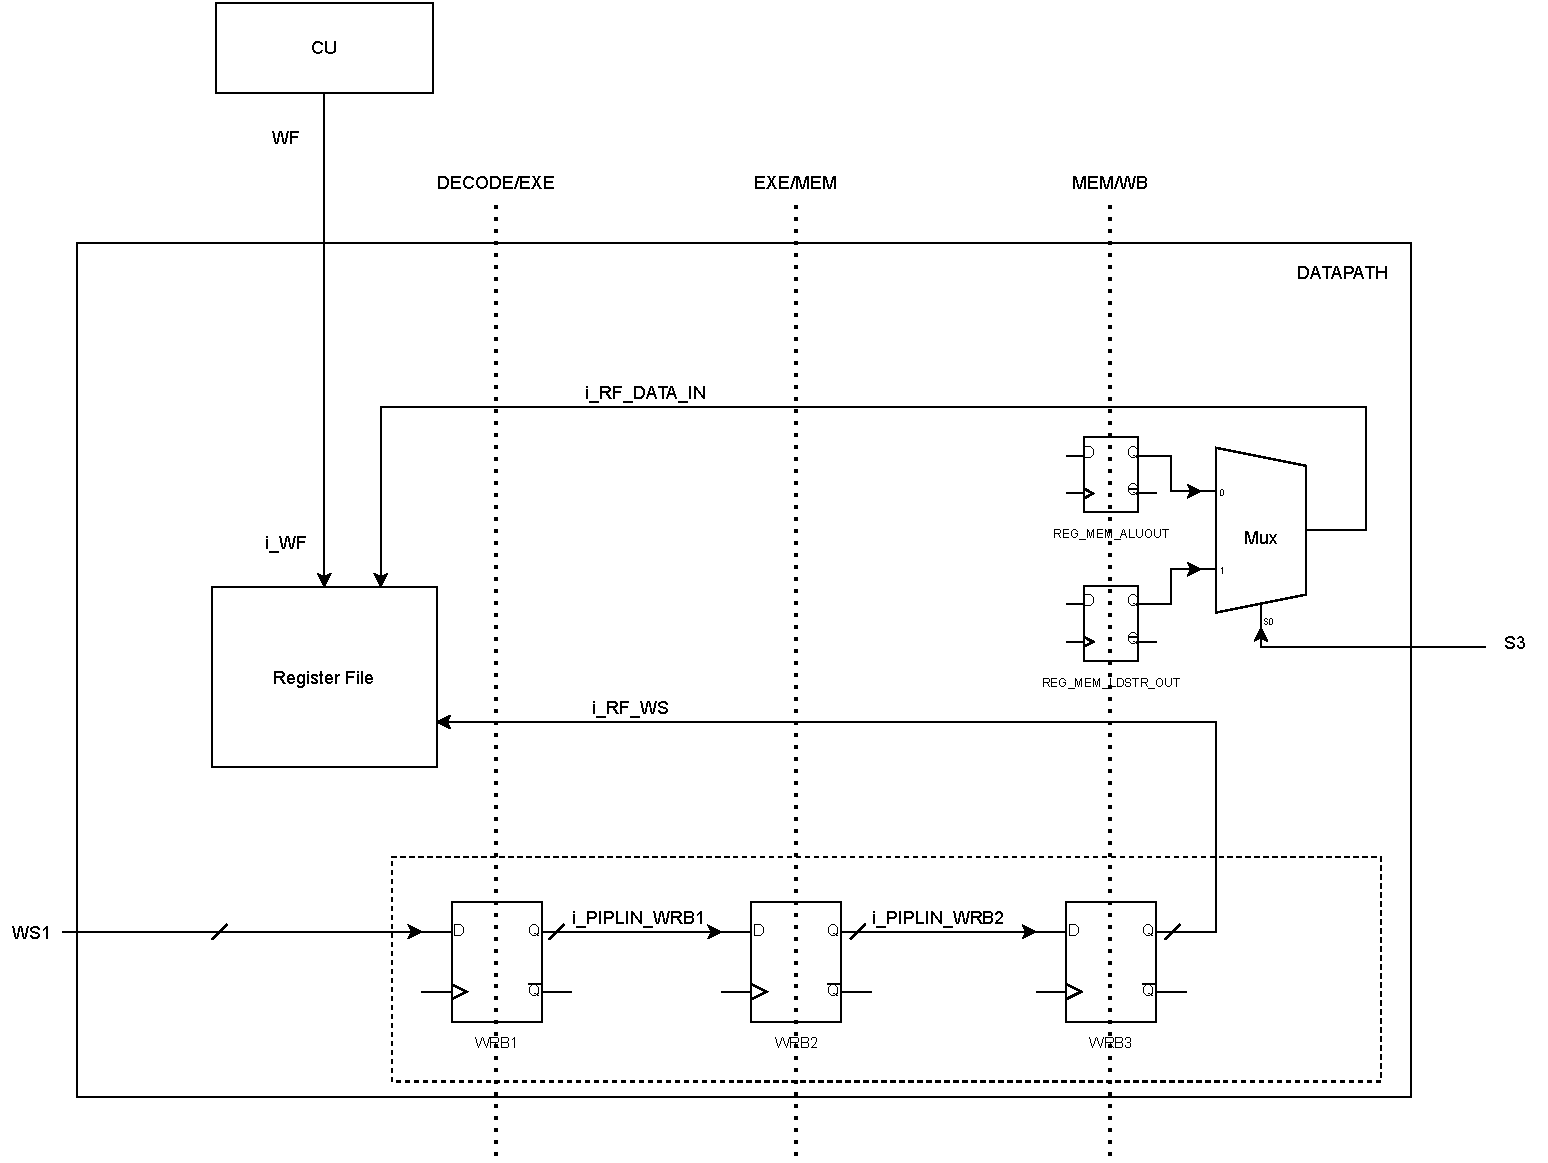
\includegraphics[width=0.85\textwidth]{chapters/7_WriteBackStage/images/writeback.pdf}
    \caption{Execute stage}
    \label{fig:wb_stage}
\end{figure}
Figure \ref{fig:wb_stage} shows the simplified diagram used to delaying the destination register (\texttt{WS1}), based on three registers in the Datapath.
When the instruction reaches the Write Back stage in the pipeline, the register index on 5 bits is fed back to the write input of the Register File and an additional signal, called \texttt{WF} is used to enable the write.\newline\newline
An additional signal, called \texttt{S3}, is used to select which data to take as input for the register file. Data can come from two different sources:
\begin{itemize}
    \itemsep0sp
    \item It can take directly the output of the Load and Store unit, via the \texttt{REG\_MEM\_LDSR\_OUT} in case the selection signal \texttt{S3 = 1}
    \item It can take the output of the ALU (that includes set-cmp unit), via the \texttt{REG\_MEM\_ALU\_OUT} in case the selection signal \texttt{S3 = 0}
\end{itemize}

The \texttt{R0} register must be protected against the Write Back, in fact, it has to be always 0. For this reason, a masking procedure has been implemented in order to solve this problem. The \texttt{WF} signal is gated with a non-zero check over the \texttt{i\_RF\_WS} signal; in few words, the write enable signal is set to 0 if a write on \texttt{R0} is requested.

\hfill
\begin{lstlisting}[style=vhdl,caption={VHDL code gating for the WS signal coming from the CU}]
    i_WF <= WF when (TO_INTEGER(unsigned(i_RF_WS)) /= 0) else '0';
\end{lstlisting}